\chapter{Using Logic ICs}
\label{chapLogicICs}

% FIXME - introduce the concept of inverted and make it a glossterm

In Chapter~\ref{chapIC}, we worked with our first Integrated Circuit, the LM393 Voltage Comparator.  
In this chapter, we are going to look at other ICs and talk more about how they are named and used in electronics.

\section{Logic ICs}

One of the easiest class of ICs to use are the \emph{logic} ICs.  
A logic IC is a chip that implements a basic function of \glossterm{digital logic}.
In digital logic, electric voltages are given meanings of either ``true'' or ``false,'' usually with ``false'' being a voltage near zero, and ``true'' being a positive voltage (often between 3--5 volts).
These values are also referred to a 1 (for true) and 0 (for false), or HIGH (for true) and LOW (for false).
Then, the digital logic ICs implement logic functions that combine different signals (usually designated as A and B) and give an output signal (usually designated as Y or Q).

For instance, the \glossterm{AND} function will output a ``true'' (positive voltage) value if both of its inputs are true, and will output a ``false'' (near-zero voltage) value otherwise.  
In other words, if A \emph{and} B are true, Y is true.
As another example, the \glossterm{OR} function will output a ``true'' value if either of its inputs are true.
In other words, if A \emph{or} B are true, Y is true.
Figure~\ref{figTruthTable} shows the most common types of logic operations and how they work.

\begin{figure}
\caption{Common Logic Operations}
\centering
\label{figTruthTable}
\begin{tabular}{l | l | l| | l}
\textbf{Operation} & \textbf{A} & \textbf{B} & \textbf{Y} (output) \\
\hline
AND & false & false & false \\
AND & false & true & false \\
AND & true & false & false \\
AND & true & true & true \\
\hline
OR & false & false & false \\
OR & false & true & true \\
OR & true & false & true \\
OR & true & true & true \\
\hline
XOR & false & false & false \\
XOR & false & true & true \\
XOR & true & false & true \\
XOR & true & true & false \\
\hline
NOR & false & false & true \\
NOR & false & true & false \\
NOR & true & false & false \\
NOR & true & true & false \\
\hline
NAND & false & false & true \\
NAND & false & true & true \\
NAND & true & false & true \\
NAND & true & true & false \\
\hline
NOT & false & N/A & true \\
NOT & true & N/A & false \\
\end{tabular}
\end{figure}

As we have seen, AND yields a true result when both A and B are true and OR yields a true result when either A or B are true.
So what are the others?
\glossterm{XOR} is \emph{exclusive OR}, which means that it is just like OR, but is also false when both inputs are true.
\glossterm{NOR} is \emph{not OR}, which means that it is the exact opposite of OR.
Likewise, \glossterm{NAND} is \emph{not AND}, which means that it is the exact opposite of AND.
Finally, \glossterm{NOT} only has one input, and simply reverses its value.

Each digital logic function, when implemented in electronics is called a \glossterm{gate}.
The nice thing about building circuits with logic gates is that, rather than using math, you can build circuits based on ordinary language.
If you were to say, ``I want my circuit to output a signal if both button 1 \emph{and} button 2 are pressed,'' then it is obvious that you would use an AND gate to accomplish this.

\simplegraphicsfigure{The Pinout of a CD4081 Chip}{CD4081Pinout}{0.16}

Most logic gates are implemented in chips that contain multiple (often four) implementations of the same gate.
For instance, the CD4081 chip is a quad NAND gate chip.
The pinout for this chip is shown in Figure~\ref{figCD4081Pinout}
Note that it has a supply voltage pin (pin 14) as well as a ground pin (pin 7) to supply power to all the gates on the chip.
Each logic gate is numbered 1--4 and the inputs are labelled A and B with the output of Y.

To use the chip, you pick which one of the four gates you are going to use (it doesn't really matter which).
If we want to use Gate~1, then we put our inputs on 1A and 1B and then our output signal goes to 1Y.
Note that, unlike the IC from the last chapter, this logic gate has a powered output---it actually supplies voltage and current to drive a (small) output signal.

Logic gates are wired to expect relatively fixed, predefined voltages on their inputs, and output the same voltage levels.
They do not need current-limiting resistors for their inputs because the inputs themselves are usually high-resistance (i.e., $1,000,000--10,000,000\myohm$).
Because of the high resistance on the inputs, it also means that even if there is a resistor on the input, it will not affect the input voltage significantly (think of a voltage divider with $1,000\myohm$ for the first resistor and $10,000,000\myohm$ for the second resistor---the voltage will not change much after the first resistor).
It also means that the current going into the gate is essentially ignorable ($I = \frac{V}{R} = \frac{5}{10,000,000} = 0.0005\mymamp$).

For some logic chips, the input voltage is expected to be around $3.3\myvolt$ or $5\myvolt$, while as for others it is based on the supply voltage.
However, nearly all ICs are limited in how much current they can put out before they fry.  
This is usually somewhere in the range of $8--20\mymamp$, depending on the chip.
Because of this, if you use a logic gate to directly power a device (such as an LED), you probably will need a current limiting resistor to keep the output current down below these limits.

There are logic chips that have open collector outputs (like the LM393 from Chapter~\ref{chapIC}), but they are more rare because they are harder to use.

\simplegraphicsfigure{Example Circuit Using an AND Gate}{LogicGateExample}{0.08}

Lets say that we want to build a circuit which will turn on an LED if \emph{both} of two buttons are pushed at the same time.
Figure~\ref{figLogicGateExample} shows a circuit to accomplish this.
It has two buttons, one wired to 1A (pin 1) and one wired to 1B (pin 2).
The output 1Y (pin 3) then goes to an LED with a current limiting resistor.
You may wonder what the resistors attached to the buttons are doing.
Those will be explained in Section~\ref{secPullDownResistors}.

For most logic chips, the manufacturers recommend that unused inputs (but not outputs!) be connected to ground. 
This makes the chip more efficient in power consumption, but for simple projects like these it isn't really necessary.
If you wish to connect the unused inputs to ground then it is a better circuit design.

Note that the circuit shows a $5\myvolt$ source.
While the CD4081 is tolerant of a wide range of input voltages and would operate just fine at $9\myvolt$, many digital logic chips are not.
Many digital logic chips operate at pre-specified voltages, usually either $5\myvolt$ or $3.3\myvolt$.
Therefore, we will take a moment and look at how we can get an input source for a specific voltage.

\section{Getting a $5\myvolt$ Source}

So far in this book, however, we have mostly dealt with $9\myvolt$ batteries.
However, digital logic circuits often operate at lower voltages (usually $5\myvolt$ or $3\myvolt$).

Therefore, we need to find a way to convert a $9\myvolt$ source into a $5\myvolt$ source.
There are several options for doing this, all depending on your requirements and/or the supplies you have available to you.

One option is to build a simple $5\myvolt$ power supply using the knowledge you already have.
In Chapter~\ref{chapBasicResistorCircuits} we showed how to build a voltage divider to step down the voltage from a higher voltage source to a lower one.
Although not ideal, this could work fine for simple test circuits.
A better option would be to build the Zener diode voltage regulator that was shown in Chapter~\ref{chapDiodes} if you have a $5\myvolt$ Zener diode handy.

\simplegraphicsfigure{A 7805 Voltage Regulator in a To-220 Package}{TO220Pkg}{0.08}

Another option is to use a voltage regulator IC.
The LM7805 is a simple voltage regulator circuit you can use to convert a $9\myvolt$ voltage source (or higher--up to $24\myvolt$) into a $5\myvolt$ voltage source with minimal current loss.
It is itself an IC, though with a different kind of packaging than we've seen, known as a \glossterm{TO-220 package}.
You can see what this looks like in Figure~\ref{figTO220Pkg}.
On these packages, if you are reading the writing on the package, pin 1 (input voltage) is on the left, pin 2 (ground) is in the middle, and pin 3 (output voltage) is on the right.
Figure~\ref{figVoltageRegulatorLogicGate} shows what this looks like in a circuit diagram.

\simplegraphicsfigure{Logic Gate Circuit with a Voltage Regulator}{VoltageRegulatorLogicGate}{0.08}

\simplegraphicsfigure{Simple Way to Attach the LM7805 to Your Breadboard}{LM7805Breadboard}{1}

Figure~\ref{figLM7805Breadboard} shows how to attach the LM7805 regulator to your breadboard.
First, plug the regulator into your breadboard so that each pin is on its own terminal strip.
Next, plug the positive wire from the battery into the terminal strip with the voltage regulator's pin 1 and the negative wire from the battery to the negative/ground power rail on the breadboard.
Then, connect the voltage regulator's pin 2 (ground) to the negative/ground power rail. 
Finally, connect the voltage regulator's pin 3 (output voltage) to the positive power rail.
You now have a $5\myvolt$ supply!

Note that some LM7805s have pins that are too big for breadboards.
That's unfortunate, but they are pretty rare.  
As long as you buy from companies that target hobbyists, you are likely to get a component that will work well with breadboards.

Another option for $5\myvolt$ power is to use an add-on unit for your breadboard.
There are many full-featured power units available for use in standard breadboards (unfortunately, there is no standard name or part number for these units, so we will just call them \emph{breadboard power units}).
This type of unit plugs into the power rails of your breadboard, and can output either $5\myvolt$ (the logic voltage we are using here) or $3.3\myvolt$ (another popular logic voltage).
The breadboard power unit can take voltage from a variety of sources, including batteries (with a compatible plug), a wall outlet (with an appropriate adapter), or even with USB power (either from your computer or a wall charger).
To use the breadboard power unit, be sure the jumpers are set to the correct output voltage, and be sure to plug it in to your breadboard in the correct direction.  
There is also an on/off switch provided in most such units so that you don't have to wire one yourself.
The breadboard power unit has positive/negative markings, so be sure they line up with the positive/negative markings on your breadboard.

\fixme{Show a photo of the power unit}

For the rest of the book, if the schematic requests a voltage other than $9\myvolt$, feel free to use any of these methods to supply the proper power to your projects.

\section{Pull-Down Resistors}
\label{secPullDownResistors}

In Figure~\ref{figLogicGateExample}, we looked at the circuit diagram for a simple AND gate.  
We noted that each button had a resistor connecting it to ground, but we did not mention why.
In digital logic circuits, buttons and single-pole switches, when they are open, essentially disconnect the circuit.
Because the inputs are high-resistance inputs (i.e., they use very little current), simply disconnecting the input circuits is not always enough to turn them off!
Think of it this way---when you connect the circuit by pushing the button, the whole wire becomes positive.
When you let go of the button, the state of the wire has not changed.
Eventually the positive charge will drain out through the gate, but, since the input uses so little current, it will take a while for that to happen.
Therefore, we have to provide another path for the electricity to go when the button is not pressed.
Note that some logic chips actually supply pull-up resistors internally which make the inputs always positive when disconnected.  
In those cases, the pull-down resistor does essentially the same job, but is even more necessary than before.

These resistors are called pull-down resistors because, when the button circuit is not connected, they pull the voltage level down close to zero through the resistor.
The resistor is very important because, when the button is connected, it keeps the voltage high and limits the amount of current that leaks out across the resistor.
If you directly connected the button to ground without the resistor, then pushing the button would not raise the voltage because it is still directly connected to ground, and would therefore remain at zero volts.  
Having the resistor there makes sure that the voltage on the inputs remains high while the button is pressed, and bleeds off when the button is released.

In short, without a path to ground, when you let go of the button, the input could remain high.
However, without the resistor, pushing the button would cause a short-circuit.
Therefore, a pull-down resistor allows voltage to drain off quickly when the button is not pressed, but also prevents disasters and wasted current when the button is pressed.

The value of a pull-down resistor is usually somewhere between $1\mykohm$ and $10\mykohm$.  
Beyond $10\mykohm$ the actual function of pulling the voltage down to zero can be slowed down.  
Additionally, even above $4\mykohm$ it is possible to interfere with the actual logic operation of the chip.
Having a resistor below $1\mykohm$, however, means that you are just wasting current.

So, for any button-type input to a digital logic circuit (where the circuit is \emph{phyiscally disconnected} when the input is off), a pull-down resistor is needed to make sure that the input \emph{actually} goes low when the circuit disconnects.

\section{Combining Logic Circuits}

Logic chips that operate at the same voltage are very easy to combine together.
Let's say that you had three buttons that you wanted to monitor, and you wanted the light to come on if someone pushed either buttons 1 \emph{and} 2 together \emph{or} button 3 (or all of them).
To do that, you would need an AND gate and an OR gate.
Buttons 1 and 2 would be wired with the AND gate, and button 3 would be combined with the output of the AND gate through an OR gate.

\simplegraphicsfigure{Multiple Logic Gates Combined in a Circuit}{MultipleGates}{0.08}

Figure~\ref{figMultipleGates} shows what this looks like.
Since there are so many voltage/ground connections, the figure does not have an explicit battery drawn, instead it simply shows $+5\myvolt$ wherever it should connect to the voltage source, and a ground symbol wherever it should connect to the battery negative.
As you can see here, there are two logic ICs---the CD4081 having the AND gate and the CD4071 having the OR gate.
The output of the first AND gate is wired into one of the inputs of the OR gate.

This works because, unlike the LM393 (discussed in Chapter~\ref{chapIC}), these logic gates actually supply output voltage and current as well.  
Because the inputs to the logic gates are high-resistance, there is no need for a current-limiting resistor when combining gates in this way.

Now, it is fine to draw logic circuits the way we have in Figure~\ref{figMultipleGates}.
However, as the logic becomes more complex, actually drawing all of the connections to voltage and ground become tiring, and trying to get all of the wires to the right spot on the chip can get messy as well.
Because of this, engineers have devised a simpler way of describing logic gates and logic circuits.

\simplegraphicsfigure{Logic Gates Represented as Shapes Instead of IC Pins}{MultipleGatesShapes}{0.08}

Instead of representing the entire chip on a schematic, engineers will represent only the logic gates themselves.
Additionally, since the power goes to the whole chip (and not the individual gates), in such a drawing the power connections for the gates are not shown.
The standard that was developed represents each type of gate with a shape.
Figure~\ref{figMultipleGatesShapes} shows what this circuit drawing looks like if it is drawn using shaped gates instead of IC pins.
The actual physical circuit is the same, this is only to simplify the schematics to make them easier to understand and follow.

\simplegraphicsfigure{Common Gates Used in Schematic Drawings}{CommonGates}{0.08}

Figure~\ref{figCommonGates} shows what these gate drawings look like.
The AND gate has a flat back panel and a simple, rounded front.
The OR gate looks a bit like a space shuttle, with both the back and the front angled.
The NOT gate is a triangle with a circle at the tip.
This circle can also be added to other gates to show that the gate is the opposite one.
For instance, a NAND gate is drawn by first drawing an AND gate, and then adding a circle to the front, indicating that the gate behaves like an AND gate with a NOT gate in front of it.
Similarly, the NOR gate is an OR gate with a circle in front of it.
The XOR gate is similar to the OR gate, but with an extra line going across its inputs.

Many times, the internal schematics of a chip are shown using gate symbols, in order to help you understand the operation of the chip and how the pins work.
For instance, Figure~\ref{figCD4081InternalLayout} shows how the CD4081 chip is wired up internally.
You can see the inputs going through the logic gate, and out towards the output.
While this isn't any new information you didn't already know, if may help you understand why the pins are laid out the way that they are.

\simplegraphicsfigure{The Internal Layout of the CD4081}{CD4081InternalLayout}{0.08}

As an interesting side-note, every logic function can actually be built from NAND gates, though you have to wire them up in strange ways.
You can actually build a computer entirely from NAND gates if you wanted to.
It is not incredibly important, but Figure~\ref{figNANDLogic} shows how to build each type of logic gate from NAND gates.
As an activity, go through the truth tables in Figure~\ref{figTruthTable} and see if you can follow how each set of values becomes the result.

\simplegraphicsfigure{How Each Gate Can Be Built from NAND Gates}{NANDLogic}{0.08}

\section{Understanding Chip Names}

One of the biggest problems in learning to build electronic devices is the bewildering array of chips, each with some weird name.
``Oh, for that you want an NE555P,'' or, ``You could use a SN74HC00P or a CD4011BE for that task.''
What language are such people speaking?

There is a huge selection of chips available, and learning their names is a daunting task.
Appendix~\ref{appICNaming} attempts to offer some method to the madness, but, at the end of the day, chip names are like people's names---you get to know them by using them.
Nobody knows everybody's name, but, for the types of projects you like to work on (whatever that happens to be), there will be standard chips whose names you will eventually come to know.

Once you make it through this book, you should have a solid enough background to search for the chips you need, have some understanding of the part names, and be able to find the chips you need for your projects.
If you buy the chips from a seller geared towards amateurs and hobbyists, they will likely also include tutorials and additional information available in an easier-to-understand format than just datasheets.

% FIXME - refer questions to a forum

\reviewsection

In this chapter, we learned:

\begin{enumerate}
\item A logic IC implements basic digital logic functions such as AND, OR, NOT, etc.
\item These logic functions refer to essentially the same ideas that they mean in ordinary language, and exactly what they mean in formal logic.
\item Logic ICs use different voltage levels for true and false---usually with true being near the supply voltage and false being near zero voltage.
\item True is sometimes referred to as HIGH or 1.  False is sometimes referred to as LOW or 0.
\item The inputs of a logic function are usually designated as A and B, and the output is usually designated as Y or Q.
\item A single digital logic function is called a gate.  Most logic ICs have more than one gate on a single chip.
\item Logic ICs require a supply voltage and a ground connection to power the logic.
\item Most logic ICs provide powered logic outputs, so that a ``true'' value supplies both voltage and a small amount of current on its output.  However, a current-limiting resistor is usually required.
\item If an input to a logic IC may be disconnected for its ``false'' state (as is common with button inputs), then it needs a pull-down resistor to connect it to ground when the button is not being pushed.
\item Logic ICs can usually be combined by wiring the output of one to the input of another to create more complex logical conditions.
\item Logic gates are often drawn in schematics using basic shapes to indicate their operation, rather than as connections to chips.  In these cases, the power connections are not shown by schematics.
\item Every logic gate can actually be built from NAND gates wired together.
\item IC names are very confusing and take time and experience to get to know them well.
\item Many ICs require specific voltage levels to operate, often at $5\myvolt$ or $3.3\myvolt$.
\item Many solutions are available for generating specific voltages, including voltage dividers, zener diodes, voltage regulators, and add-on breadboard power units.
\item The LM7805 is a very common $5\myvolt$ voltage regulator.
\end{enumerate}

\applysection


\begin{enumerate}
\item 
\question{Draw the circuit in Figure~\ref{figLogicGateExample} yourself.  Identify the function of each resistor.}
\solution{
The circuit is repeated below:
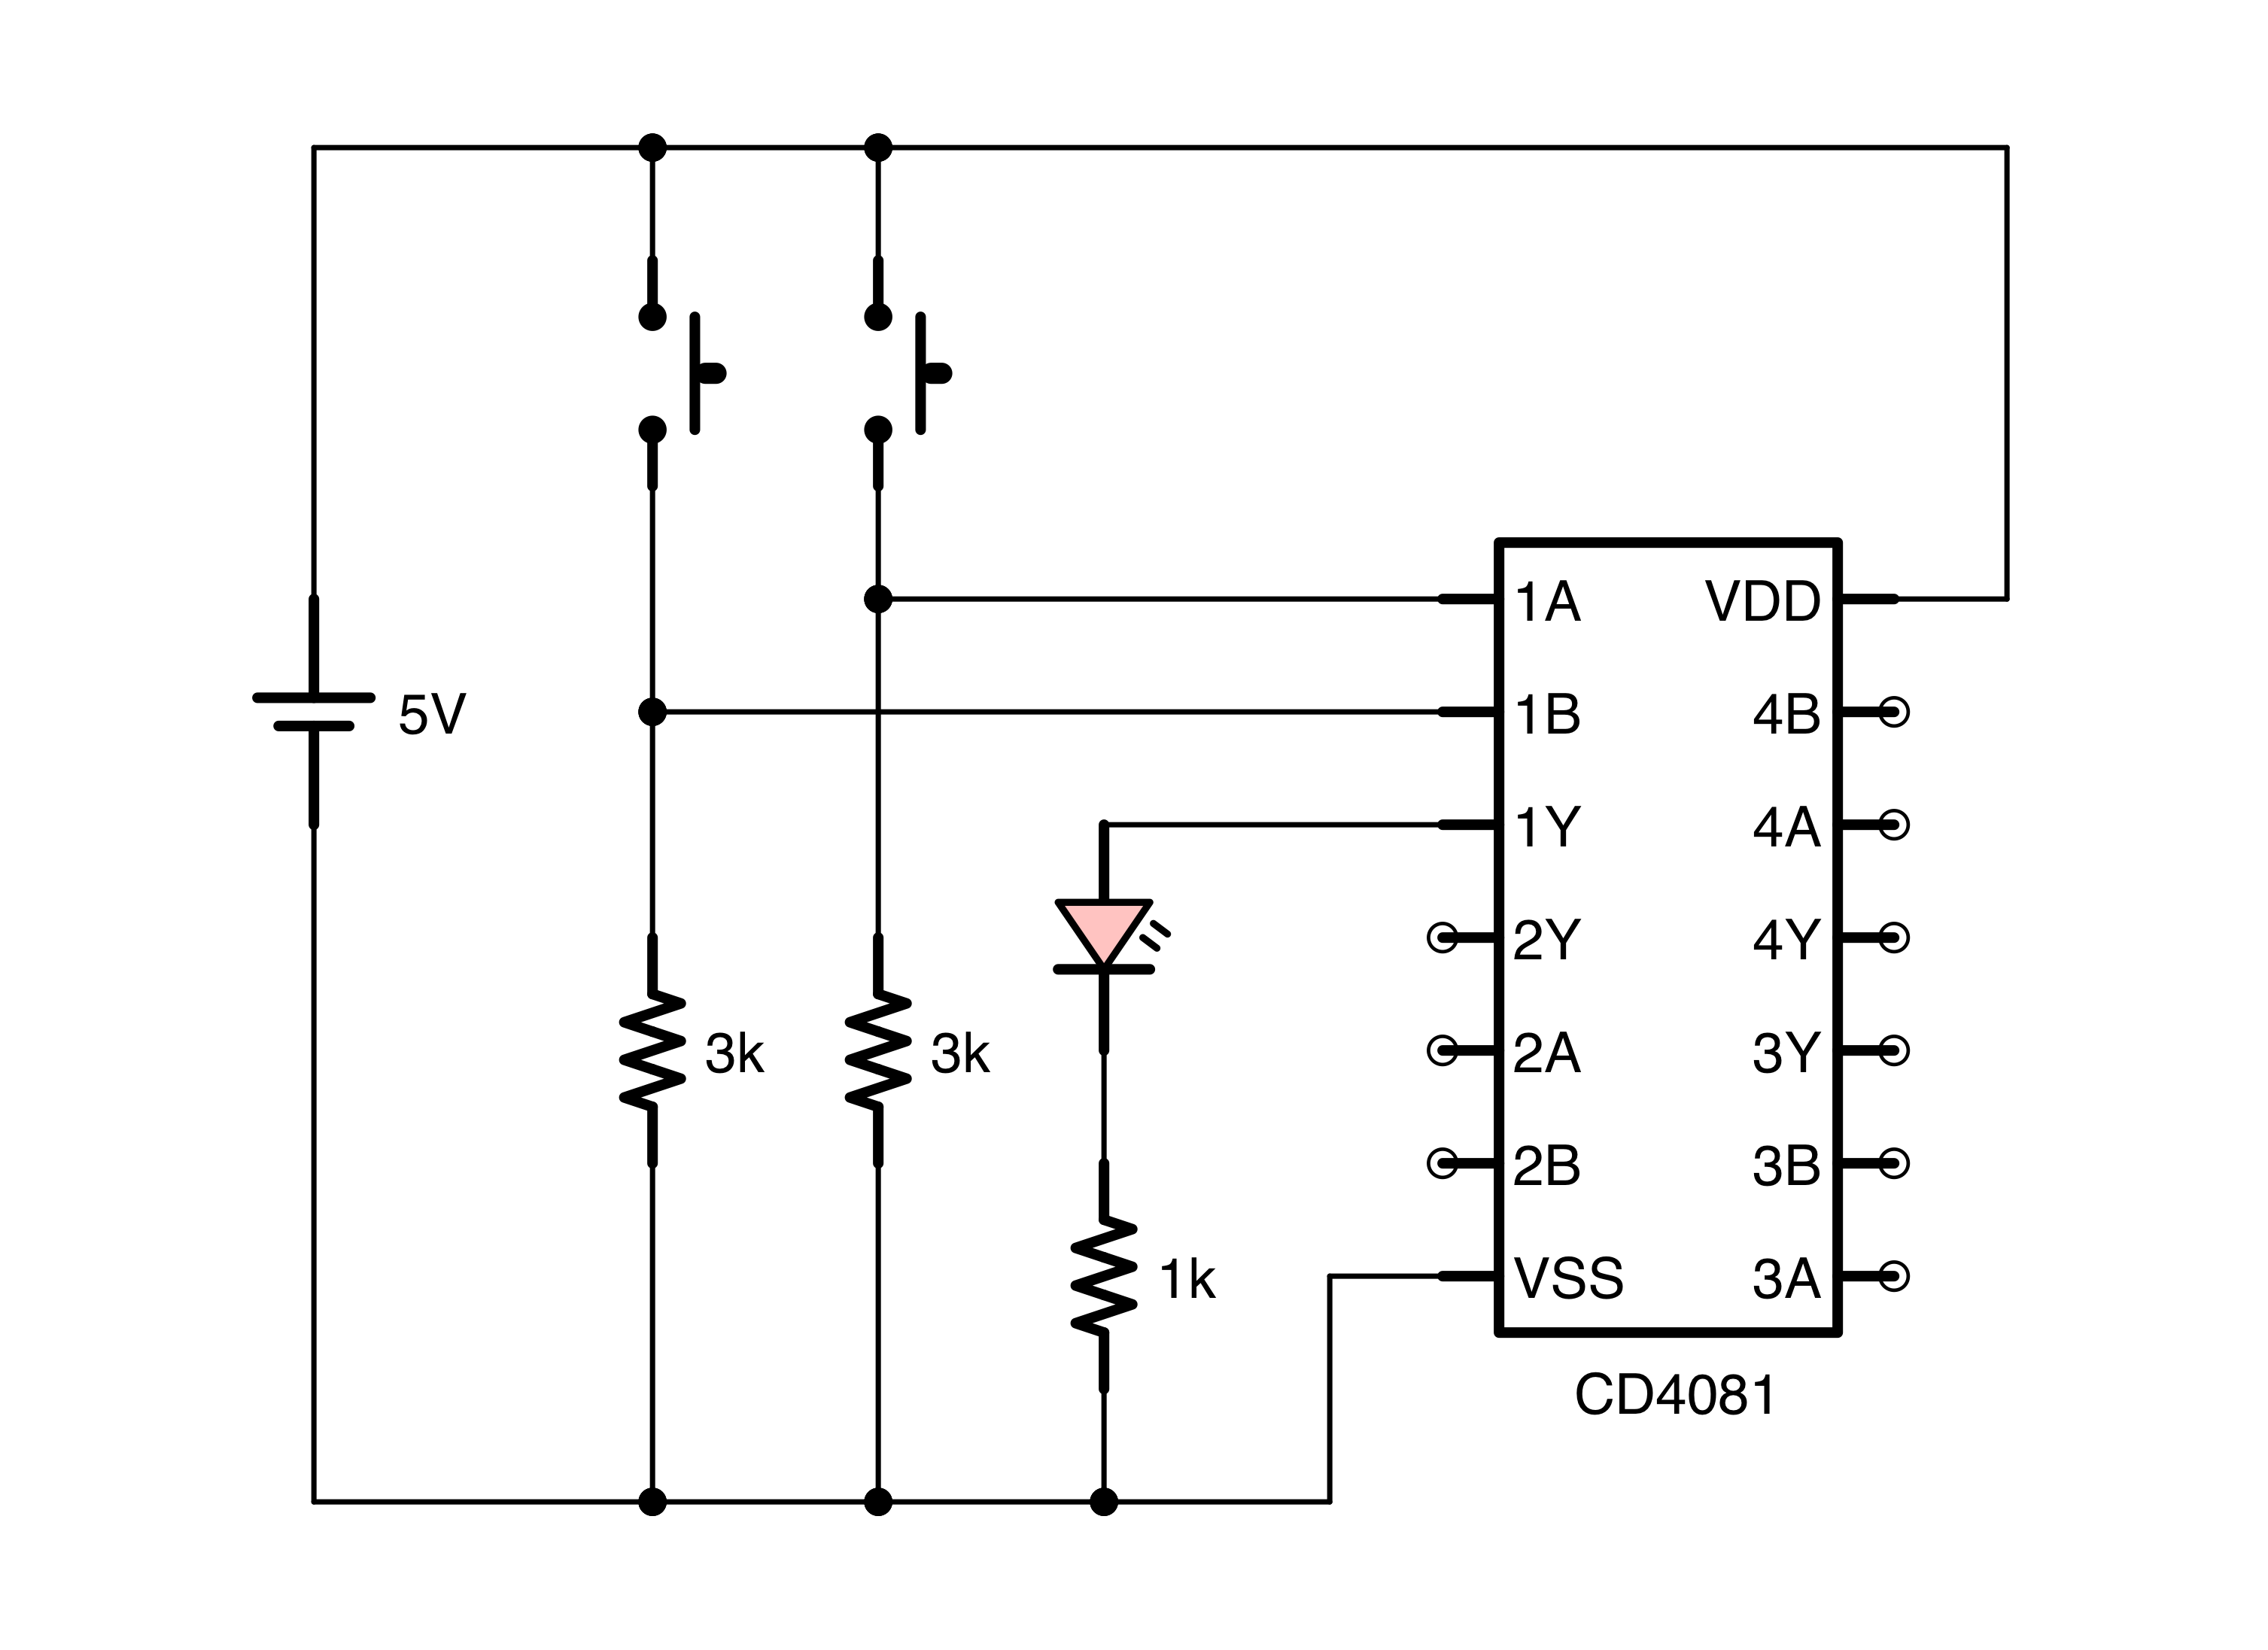
\includegraphics[width=\columnwidth]{LogicGateExample.png}

The 3k resistors are pull-down resistors.  The 1k resistor is a current-limiting resistor for the LED.
}
\item 
\question{Build the circuit in Figure~\ref{figLogicGateExample} (don't forget that the power source should be $5\myvolt$).}
\solution{When built, the circuit should only light up the LED when \emph{both} the buttons are pushed down.}
\item 
\question{If you assume that a negligible amount of current flows through the inputs of the AND gate, and that the output functions as a $5\myvolt$ voltage source (and the LED is red), how much current flows through each resistor when all of the buttons are pressed?  What, then, is the total current used by the circuit if you ignore the logic gate?}
\solution{The pull-down resistors each have $1.67\myamp$ of current, and the current-limiting resistor has $3.2\mymamp$ of current.  Therefore, the total current is $6.54\mymamp$.}
\explanation{When a button is pressed, there is a $3,000\myohm$ pull-down resistor connecting the power to ground.
Therefore, we can use Ohm's Law to find the current usage:
\begin{align*} 
I &= V / R \\
  &= 5 / 3,000 \\
  &= 0.00167\myamp = 1.67\mymamp
\end{align*}
Therefore, \emph{each} of the button circuits are using this amount of current.

Then, when both the inputs are positive, the output goes to $5\myvolt$.
This is dropped $1.8\myvolt$ by the red LED, leaving $3.2\myvolt$ for the resistor.
Therefore, the current going through the resistor is:
\begin{align*}
I &= V / R \\
  &= 3.2 / 1,000 \\
  &= 0.0032\myamp = 3.2\mymamp
\end{align*}
Therefore, the total amount of current in this circuit is $1.67 + 1.67 + 3.2 = 6.54\mymamp$.
}
\item 
\question{Measure the actual current that flows through each resistor.  If you are having trouble pushing the buttons while you measure the current, just replace the buttons with wires for this test.}
\solution{Your currents should roughly match the answers to the previous question.}
\item 
\question{Measure the current that it used by the AND gate itself.  You can do this by measuring the supply current of the AND gate.  Measure it both when its output is true and false.}
\solution{This measurement will vary depending on the brand of AND gate you are using.  However, usually it is less than $1\mymamp$ when the output is off.  It should increase by about the output current ($3.2\mymamp$) when the output is on.}
% FIXME - stopped adding solutions here.
\item 
\question{Draw a schematic of a circuit that has two buttons (B1 and B2) which light up an LED if either button is pressed.  Use the logic gate shapes for the schematic.}
\item 
\question{Draw a schematic of a circuit that has two buttons (B1 and B2) which light up an LED if neither button is pressed.  Use the logic gate shapes for the schematic.}
\item 
\question{Draw a schematic of a circuit that has four buttons (B1--B4) which light up an LED if either B1 and B2 are pressed or if B3 and B4 are pressed.  Use the logic gate shapes for the schematic.}
\item 
\question{Look at the construction of the different gates from NAND gates in Figure~\ref{figNANDLogic}.  Copy down the OR gate construction four times, and trace how the output is generated for each possible set of inputs (true/true, true/false, false/true, false/false).  Show the inputs and outputs on each NAND gate.  Compare the outputs to the truth table for the OR function in Figure~\ref{figTruthTable}.}
\item 
\question{Take the circuit in Figure~\ref{figLogicGateExample} and draw a schematic to use pull-up resistors on the inputs rather than pull-down resistors.  How will this change the behavior of the circuit?}
\item 
\question{Let's say that we want to create a door buzzer so that someone outside a door can push a button to be let in.  However, the person inside also wants a switch to be able to disable the buzzer.  The buzzer can be thought of as a simple device that buzzes when any positive voltage is applied.  Draw a circuit diagram of this setup using logic gates.  The buzzer can be drawn as a resistor labelled ``buzzer'' (don't forget to connect the other side to ground!).}
\end{enumerate}

